\begin{center}
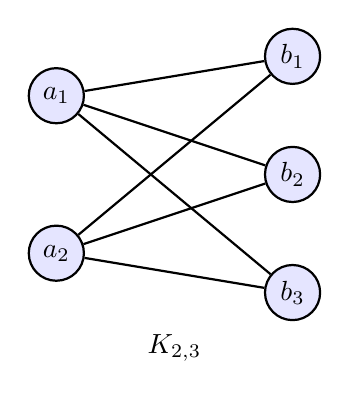
\begin{tikzpicture}[
  vnode/.style={circle, draw, minimum size=7mm, inner sep=0pt, fill=blue!10},
  thick
]
  \node[vnode] (a1) at (0, 1) {$a_1$};
  \node[vnode] (a2) at (0, -1) {$a_2$};
  
  \node[vnode] (b1) at (3, 1.5) {$b_1$};
  \node[vnode] (b2) at (3, 0) {$b_2$};
  \node[vnode] (b3) at (3, -1.5) {$b_3$};
  
  \foreach \i in {1,2} {
    \foreach \j in {1,2,3} {
      \draw (a\i) -- (b\j);
    }
  }
  \node at (1.5, -2.2) {$K_{2,3}$};
\end{tikzpicture}
\par\medskip
\textit{Obrázek 3.2: Úplný bipartitní graf $K_{2,3}$ s partitami velikosti 2 a 3.}
\end{center}